\documentclass{article}

\usepackage{amsmath}
\usepackage{amssymb}
\usepackage{mathtools}
\usepackage{fullpage}
\usepackage[T1]{fontenc}
\usepackage{lmodern}
\usepackage{tikz}
\usetikzlibrary{calc,intersections,through,backgrounds}
\usetikzlibrary{bayesnet}
\usepackage{tikzscale}
\usepackage{tkz-euclide}
\usepackage{tcolorbox}
\tcbuselibrary{skins,breakable}
% pgfplots
\usepackage{pgfplots}
\pgfplotsset{compat=1.8}
% For entities in pgfplots
\newcommand{\entpgf}[1]{\texttt{#1}}

\begin{document}

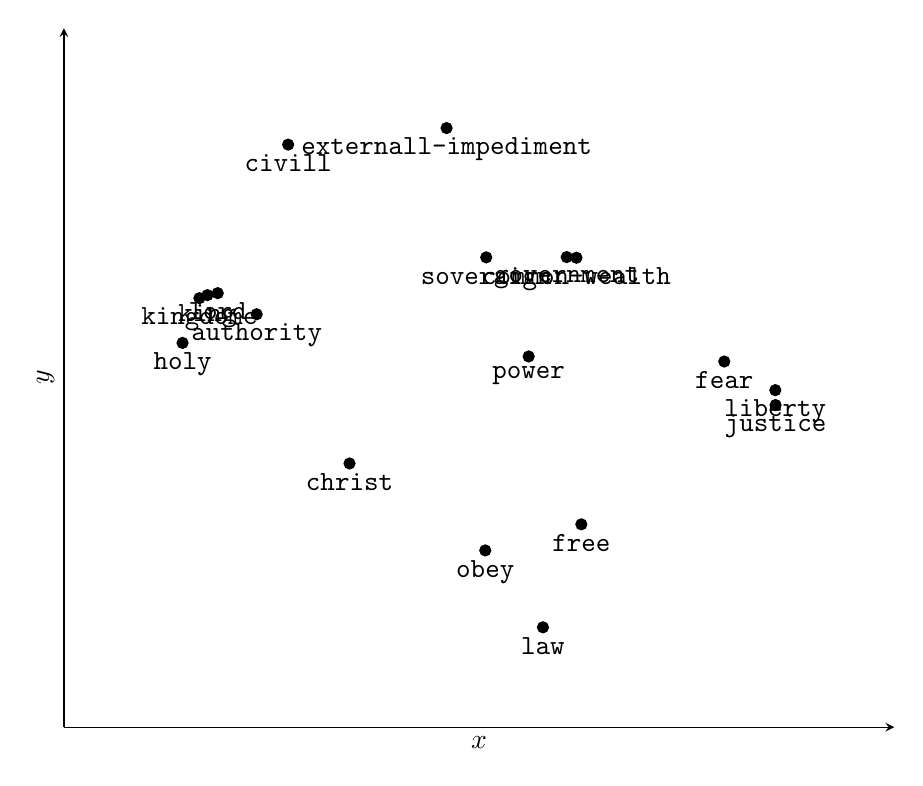
\begin{tikzpicture}
\pgfplotsset{ticks=none}
		\begin{axis}[
		    axis x line=bottom,
			axis y line=left,
			xmin=-51.98418-27.0667724609375, xmax=83.349686+27.0667724609375,
			ymin=-78.760216-32.673638916015626, ymax=84.60798+32.673638916015626,
			xtick={-51.98418,83.349686},ytick={-78.760216,84.60798},
			xlabel=$x$,ylabel=$y$,
			%x label style={anchor=west},
			%y label style={anchor=south},
			width=\textwidth
			]
			\addplot+[mark options={fill=black,color=black},only marks,point meta=explicit symbolic, nodes near coords] coordinates {
(30.26188087463379, -78.76021575927734)[]
(26.99773406982422, 9.877872467041016)[]
(17.31273078918457, 42.29462432861328)[]
(37.90427017211914, 42.17142868041992)[]
(-13.87794017791748, -25.13726234436035)[]
(-46.318809509277344, 29.94234848022461)[]
(-27.891939163208008, 79.19755554199219)[]
(-35.07691192626953, 23.684452056884766)[]
(-48.137821197509766, 28.952238082885742)[]
(17.096521377563477, -53.59331130981445)[]
(71.6435317993164, 8.220415115356445)[]
(-51.98418045043945, 14.307669639587402)[]
(35.680118560791016, 42.388587951660156)[]
(83.29209899902344, -1.1460003852844238)[]
(-43.964759826660156, 30.586462020874023)[]
(83.34968566894531, -6.031447887420654)[]
(39.021873474121094, -45.06495666503906)[]
(8.26322078704834, 84.60797882080078)[]
};
\node (law) at (axis cs:30.26188, -78.760216){};
\node (power) at (axis cs:26.997734, 9.877872){};
\node (soveraign) at (axis cs:17.31273, 42.294624){};
\node (common-wealth) at (axis cs:37.90427, 42.17143){};
\node (christ) at (axis cs:-13.87794, -25.137262){};
\node (king) at (axis cs:-46.31881, 29.942348){};
\node (civill) at (axis cs:-27.89194, 79.197556){};
\node (authority) at (axis cs:-35.076912, 23.684452){};
\node (kingdome) at (axis cs:-48.13782, 28.952238){};
\node (obey) at (axis cs:17.096521, -53.59331){};
\node (fear) at (axis cs:71.64353, 8.220415){};
\node (holy) at (axis cs:-51.98418, 14.30767){};
\node (government) at (axis cs:35.68012, 42.388588){};
\node (liberty) at (axis cs:83.2921, -1.1460004){};
\node (lord) at (axis cs:-43.96476, 30.586462){};
\node (justice) at (axis cs:83.349686, -6.031448){};
\node (free) at (axis cs:39.021873, -45.064957){};
\node (externall-impediment) at (axis cs:8.263221, 84.60798){};
\node[anchor = north, xshift=0.0, yshift=0.0] (lawl) at(axis cs: 30.26188, -78.760216){$\entpgf{law}$};
\node[anchor = north, xshift=0.0, yshift=0.0] (powerl) at(axis cs: 26.997734, 9.877872){$\entpgf{power}$};
\node[anchor = north, xshift=0.0, yshift=0.0] (soveraignl) at(axis cs: 17.31273, 42.294624){$\entpgf{soveraign}$};
\node[anchor = north, xshift=0.0, yshift=0.0] (common-wealthl) at(axis cs: 37.90427, 42.17143){$\entpgf{common-wealth}$};
\node[anchor = north, xshift=0.0, yshift=0.0] (christl) at(axis cs: -13.87794, -25.137262){$\entpgf{christ}$};
\node[anchor = north, xshift=0.0, yshift=0.0] (kingl) at(axis cs: -46.31881, 29.942348){$\entpgf{king}$};
\node[anchor = north, xshift=0.0, yshift=0.0] (civilll) at(axis cs: -27.89194, 79.197556){$\entpgf{civill}$};
\node[anchor = north, xshift=0.0, yshift=0.0] (authorityl) at(axis cs: -35.076912, 23.684452){$\entpgf{authority}$};
\node[anchor = north, xshift=0.0, yshift=0.0] (kingdomel) at(axis cs: -48.13782, 28.952238){$\entpgf{kingdome}$};
\node[anchor = north, xshift=0.0, yshift=0.0] (obeyl) at(axis cs: 17.096521, -53.59331){$\entpgf{obey}$};
\node[anchor = north, xshift=0.0, yshift=0.0] (fearl) at(axis cs: 71.64353, 8.220415){$\entpgf{fear}$};
\node[anchor = north, xshift=0.0, yshift=0.0] (holyl) at(axis cs: -51.98418, 14.30767){$\entpgf{holy}$};
\node[anchor = north, xshift=0.0, yshift=0.0] (governmentl) at(axis cs: 35.68012, 42.388588){$\entpgf{government}$};
\node[anchor = north, xshift=0.0, yshift=0.0] (libertyl) at(axis cs: 83.2921, -1.1460004){$\entpgf{liberty}$};
\node[anchor = north, xshift=0.0, yshift=0.0] (lordl) at(axis cs: -43.96476, 30.586462){$\entpgf{lord}$};
\node[anchor = north, xshift=0.0, yshift=0.0] (justicel) at(axis cs: 83.349686, -6.031448){$\entpgf{justice}$};
\node[anchor = north, xshift=0.0, yshift=0.0] (freel) at(axis cs: 39.021873, -45.064957){$\entpgf{free}$};
\node[anchor = north, xshift=0.0, yshift=0.0] (externall-impedimentl) at(axis cs: 8.263221, 84.60798){$\entpgf{externall-impediment}$};

\end{axis}
\end{tikzpicture}

\end{document}